\section{Architecture}
\brand{x-project} architecture is client-server.
The full technology stack is JavaScript based.

Server-side is based on Node.js.

\begin{description}
\itemsep1pt\parskip0pt\parsep0pt
        \item[Node.js] (\url{http://nodejs.org}) is a platform built on Chrome's JavaScript runtime for easily building fast, scalable network applications.
        \item[Express.js] (\url{http://expressjs.com}) is a minimal and flexible Node.js web application framework that provides a set of features for web and mobile applications.
        \item[Loopback] (\url{http://loopback.io}) is a set of Node.js modules to develop Web Servers applications. An application interacts with data sources through the LoopBack model API, available locally within Node.js, remotely over REST.
        \item[MongoDB] (\url{https://www.mongodb.org/}) is an open-source document database that provides high performance, high availability, and automatic scaling.
\end{description}


Client-side is based on Web Components.

\begin{description}
\itemsep1pt\parskip0pt\parsep0pt
        \item[Web Components] are a collection of standards which are working their way through the W3C and landing in browsers at the moment. In a nutshell, they allow us to bundle markup and styles into custom HTML elements.
\emph{Custom Elements}\cite{custom-elements}, \emph{HTML Imports}\cite{html-imports}, \emph{HTML Templates}\cite{html-templates}, \emph{Shadow DOM}\cite{shadow-dom}.
        \item[webcomponent.js polyfills] enable Web Components in (evergreen) browsers that lack native support.
Web Components specifications are currently W3C Working Draft, so they aren’t fully supported across all major browsers.
As these technologies are implemented in browsers, the polyfills will shrink to gain the benefits of native implementations. \cite{webcomponents-polyfills} 
        \item[Polymer library] (\url{https://www.polymer-project.org/}) provides a thin layer of API on top of web components (native implementations and their polyfills) and several powerful features, such as custom events and delegation, mixins, accessors and component lifecycle functions, that makes it easier and faster to create Web Components. Similar to \emph{Polymer} are \emph{x-tag} and \emph{Bosonic}.
        \item[iron-elements] \cite{iron-elements} is a library of utility Polymer elements from ajax requests to input elements. 
There are web repositories like \url{http://component.kitchen} and \url{http://customelements.io} that already counts thousands of open source user-contributed custom elements.
\end{description}

% \begin{figure}[!htbp]
% \centering
% 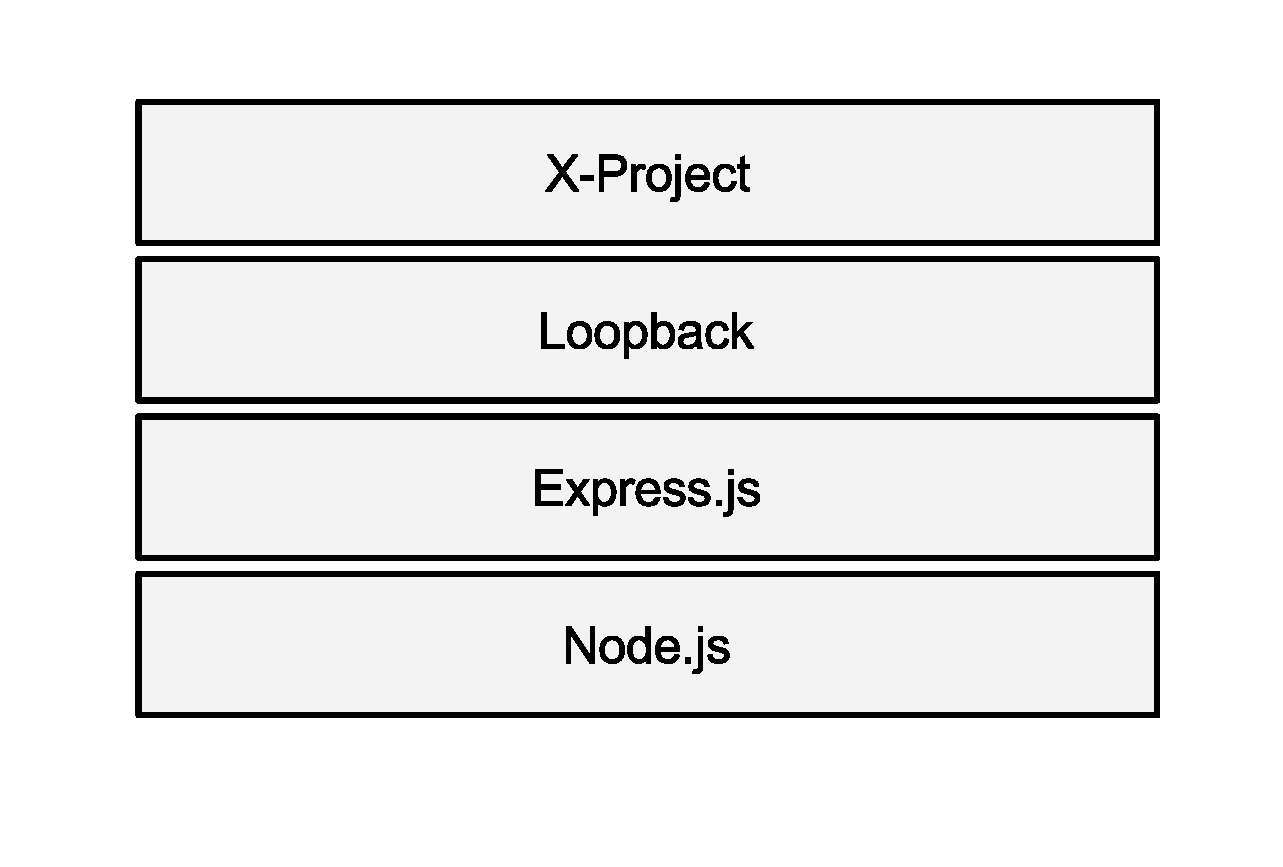
\epsfig{file=images/stack.eps, height=0.2\textwidth}
% \caption{Technology stack}
% \label{fig:tech-stack}
% \end{figure}

% \begin{figure}[!h]
%  \centering
%  \begin{subfigure}[b]{0.53\linewidth}
%  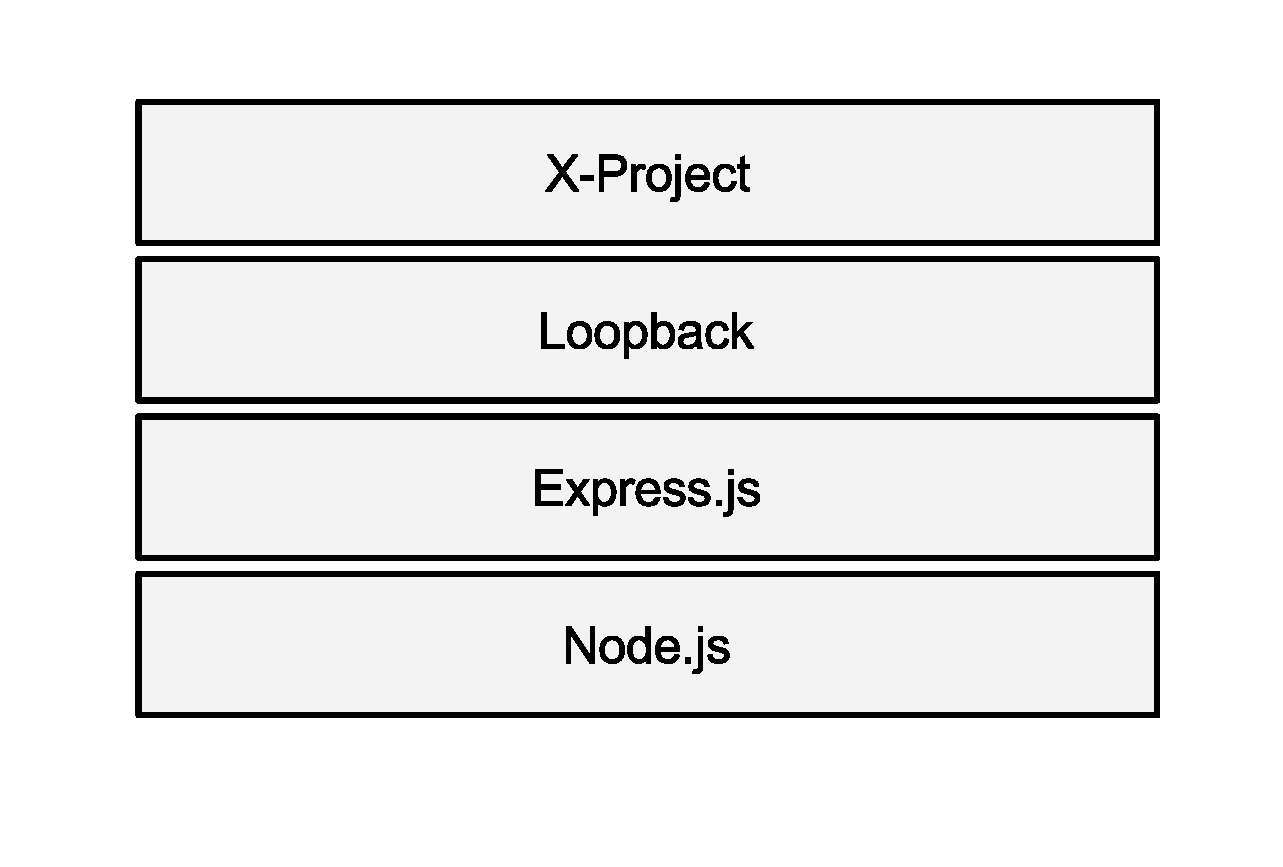
\includegraphics[width=\textwidth]{images/stack.eps} 
%  \caption{Technology stack.}
%  \label{fig:tech-stack}
%  \end{subfigure}
%  ~
%  \begin{subfigure}[b]{0.43\linewidth}
%  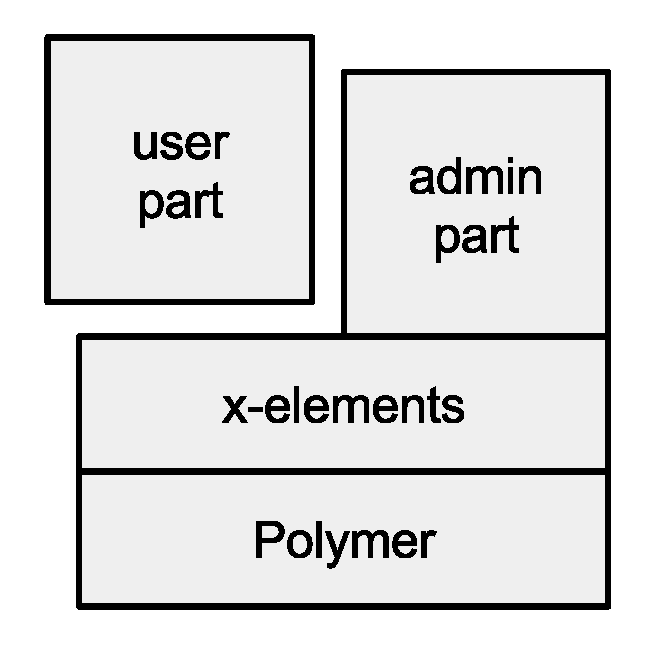
\includegraphics[width=\textwidth]{images/client-arch.eps}
%  \caption{Client-side architecture}
%  \label{fig:client-arch}
%  \end{subfigure}
 
%  % \caption{Office building: 
%  % (a) the schematic plan; 
%  % (b) the simplified 3D model generated for testing on the field 
%  % the indoor mapping project described in this paper.
%  % }
%  % \label{fig:sogei}
% \end{figure}

% \begin{figure}[!htbp]
% \centering
% 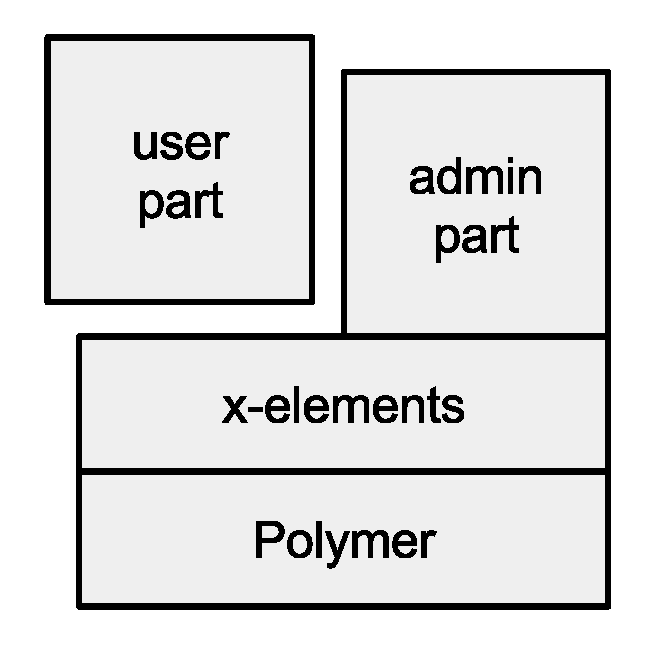
\epsfig{file=images/client-arch.eps, height=0.2\textwidth}
% \caption{Client-side architecture}
% \label{fig:client-arch}
% \end{figure}


\subsection{Server-side}
The Web Application development is document-driven.

To speed up web application development, frameworks mostly rely on external configuration files and less on procedural code \cite{6859693}.


In \brand{x-project}, server-side, the documents that drive the development are the schema of the models of the application.


These are json document. Each document represent a model and has the following fields: the \texttt{name} of the model, the set of \texttt{properties}, the list of \texttt{relations} to others models and the list of \texttt{ACL} (Access Control Layer) rules. 

\brand{x-project} (using Loopback) generates model’s API from the models schemas, to let CRUD operations on models (e.g. a model \texttt{Author} that describe a blog author generates the following HTTP RESTful API: \texttt{GET /api/authors/} to get all authors, \texttt{POST /api/authors/} to add a new author, \texttt{GET /api/authors/:author\_id} and \texttt{PUT /api/authors/:author\_id} to get (or to update) the author with id ``\texttt{author\_id}''. 
Since an blog author have blog posts (its model has a relation one-to-many to model \texttt{Post}) there are also the API to handle author's posts: \texttt{GET /api/authors/:author\_id/posts}, etc.

The API can be extended: the developer can add remote functions to models or add hooks to existing APIs to add behaviour before and/or after the API handler (to preprocess the request and/or postprocess the response).

The API are RESTful, cookie free, signed by authentication token.

\brand{x-project} applications have a built-in model that represent a user, with properties \texttt{username}, \texttt{email} and \texttt{password} for login and the property \texttt{role} used by the ACL module.
By default, only user with role \texttt{admin} can create/update/delete models in the applications.


\subsubsection{Third party services}
\brand{x-project} is designed to be connected to microservices. These tools are accessible extending the Web Application API.

An essential feature of a CMS is media storage (documents, images and videos) \cite{5552271}. 

\brand{x-project} provides a remote storage service implemented as a direct upload module to AWS Amazon S3 storage service. The media to upload don’t pass through the server but are sent directly to AWS using a signed request.
The signature of the request is provided by the module.
The module has to be configured with the AWS bucket settings: bucket name, public and secret keys. 

% \begin{figure}[!htbp]
% \centering
% 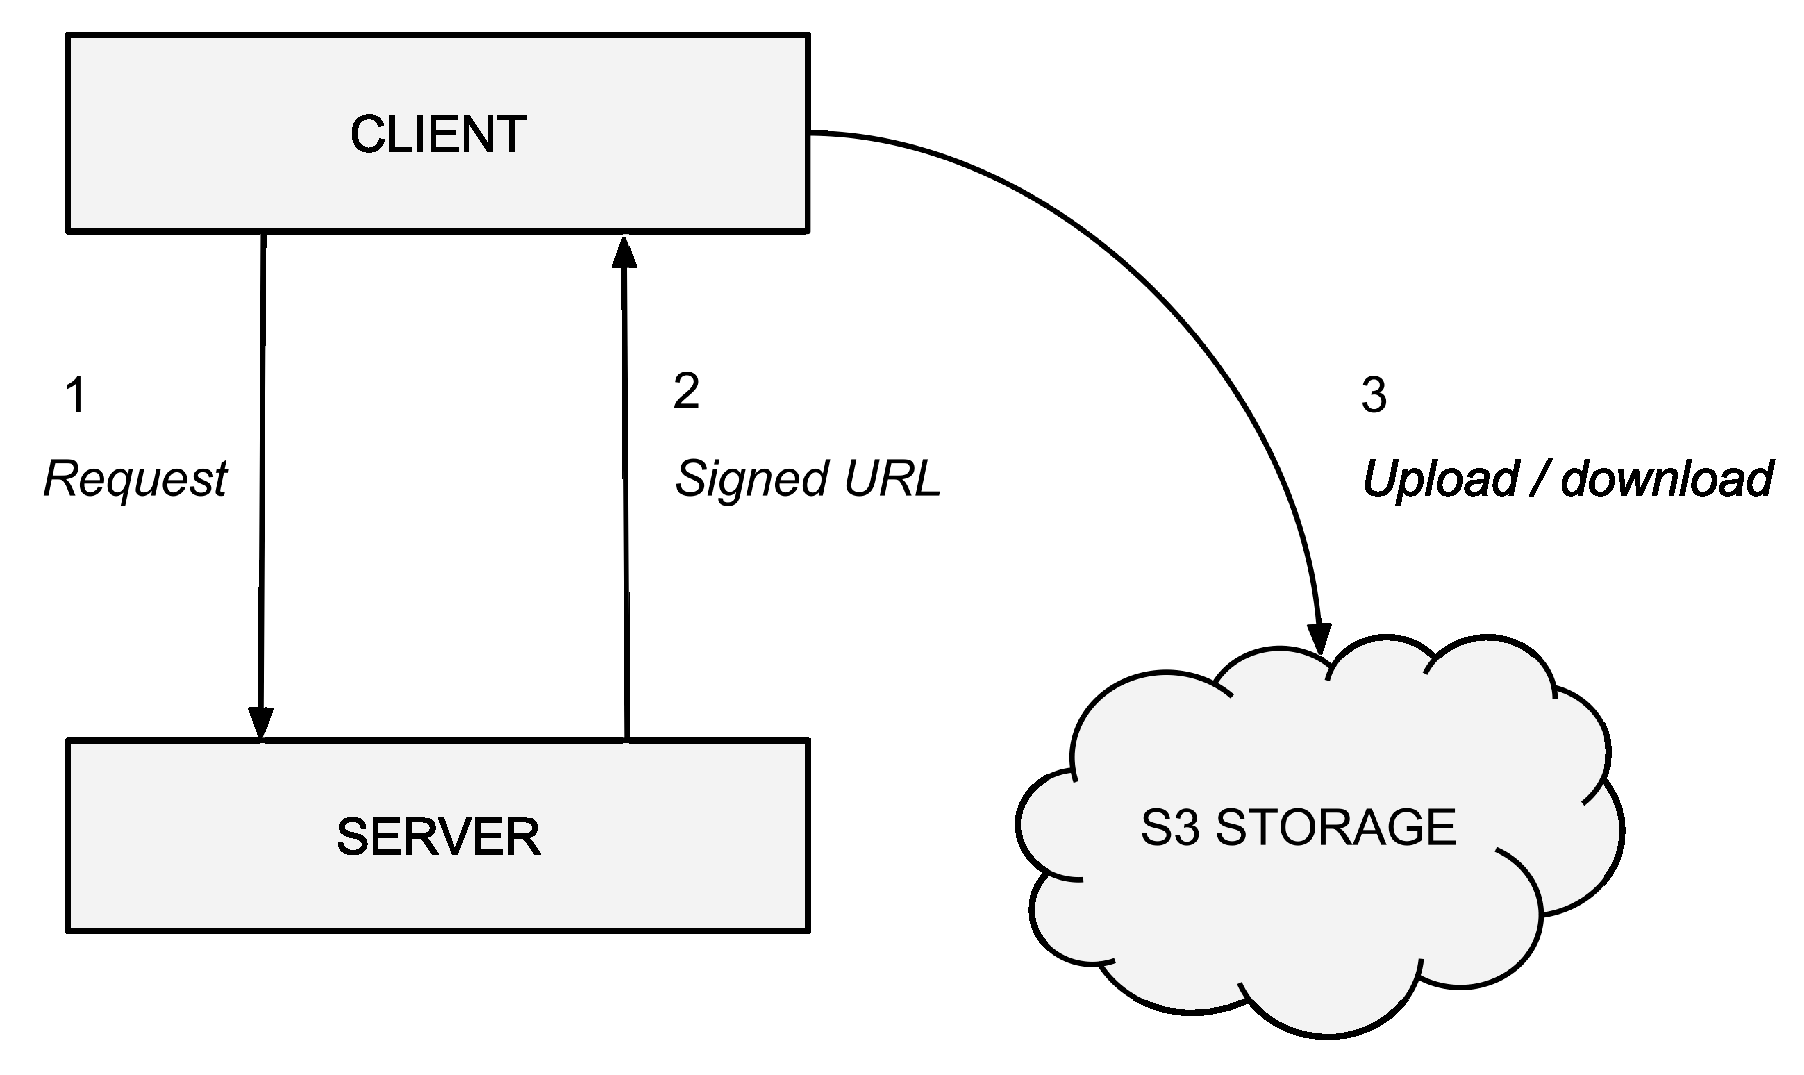
\epsfig{file=images/services.eps, height=0.24\textwidth}
% \caption{Third parties services}
% \label{fig:services}
% \end{figure}
